% =====================================================================
%  CFA Quant Awards 2026 -- Submission Paper (DRIVER)
%  Distilled from a 100+ page Master's thesis into a 5-7 page format.
%
%  Compile with: pdflatex -> bibtex -> pdflatex -> pdflatex
%  Image paths reuse the originals from the source thesis (./images/...)
% =====================================================================

\documentclass[11pt,a4paper]{article}

% --- packages --------------------------------------------------------
\usepackage[utf8]{inputenc}
\usepackage[T1]{fontenc}
\usepackage{lmodern}
\usepackage[english]{babel}
\usepackage[top=0.72in,bottom=0.78in,left=0.74in,right=0.74in]{geometry}
\usepackage{amsmath,amssymb,amsthm}
\usepackage{graphicx}
\usepackage{booktabs}
\usepackage{tabularx}
\usepackage{caption}
\usepackage{subcaption}
\usepackage{float}
\usepackage{microtype}
\usepackage{csquotes}
\usepackage[style=apa, backend=biber, natbib=true]{biblatex}
\addbibresource{00 bib.bib}
\usepackage{xurl}
\usepackage{hyperref}
\hypersetup{colorlinks=true,linkcolor=blue,citecolor=blue,urlcolor=blue}

\captionsetup{font=footnotesize,labelfont=bf,skip=3pt}
\setlength{\parskip}{0.22em}
\setlength{\parindent}{0pt}
\AtBeginBibliography{%
  \normalsize
  \sloppy
  \setlength{\itemsep}{0pt}%
  \setlength{\bibitemsep}{0pt}%
}

\begin{document}

% --------------------------- BODY ------------------------------------
\setcounter{page}{1}
% --------------------------- COVER PAGE ------------------------------
\begin{center}
    {\LARGE\bfseries Exploiting the Index Effect on the Oslo Stock Exchange Benchmark Index using Machine Learning}    
\end{center}

% --------------------------- ABSTRACT --------------------------------
\begin{abstract}
\noindent
This paper turns a well-known benchmark-rebalancing anomaly into a directly testable investment process. OSEBX, the Oslo Stock Exchange Benchmark Index, is rebuilt semi-annually from a transparent Euronext rule book. I use only the variables in that rule book--trading status, electronic-order-book turnover, free float, sector, and lagged membership--to predict index additions and deletions before the official announcement, then trade the predicted changes through active and enhanced-index portfolios. A logistic GLM and XGBoost both rank future constituents well: out-of-sample AUROC exceeds 0.97 across 26 rebalancing events from 2010 to 2023. The harder problem is economic, not statistical. A naive persistence model has 95.1\% accuracy but produces zero trades. To make the forecast investable, I introduce a conditional posterior-probability threshold that deliberately sacrifices some accuracy to increase the number of predicted changes. The best active overlays generate significant Fama--French three-factor alpha, while the risk-controlled XGBoost variant remains significant when embedded in a 2\% tracking-error enhanced-index sleeve. The central conclusion is practical: in benchmark-event trading, the useful model is not the most accurate classifier, but the classifier whose errors create a diversified and capacity-aware signal.
\end{abstract}

% --------------------------- INTRODUCTION ----------------------------
\section{Introduction}
\label{sec:intro}

Index rebalancing creates a recurring implementation problem for passive and enhanced-index investors. Once an index provider announces additions and deletions, benchmarked capital must trade in the same direction and over a narrow window. That demand pressure can move prices even when firm fundamentals are unchanged, the classic ``index effect'' of \textcite{shleifer-do-demand-curves-for-stocks-slope-down}. The effect has been documented for large global indices \parencite{lynch-new-evidence-s&p-500,afego-effects-of-changes-in-stock-index-composition} and is the empirical counterpart to the avoidable rebalancing drag estimated for benchmarked mandates \parencite{arnott-the-avoidable-cost-of-index-rebalancing}; the investment question is whether it can be forecast early enough, and cleanly enough, to be traded.

OSEBX is a useful laboratory because the index is important locally, liquid enough for institutional implementation, and transparent. Euronext selects roughly 50--80 names from the wider OSEAX universe twice per year using publicly described eligibility, turnover, free-float and sector rules \parencite{OSEBX-rule-book}. Figure~\ref{fig:idxeff} shows the economic motivation: from 2002 to 2023, future additions tended to outperform and future deletions tended to underperform before the effective date. The opportunity lies between the data cut-off date and the announcement date, when the relevant inputs are fixed but the official constituent list is not yet public.

\begin{figure}[H]
\centering
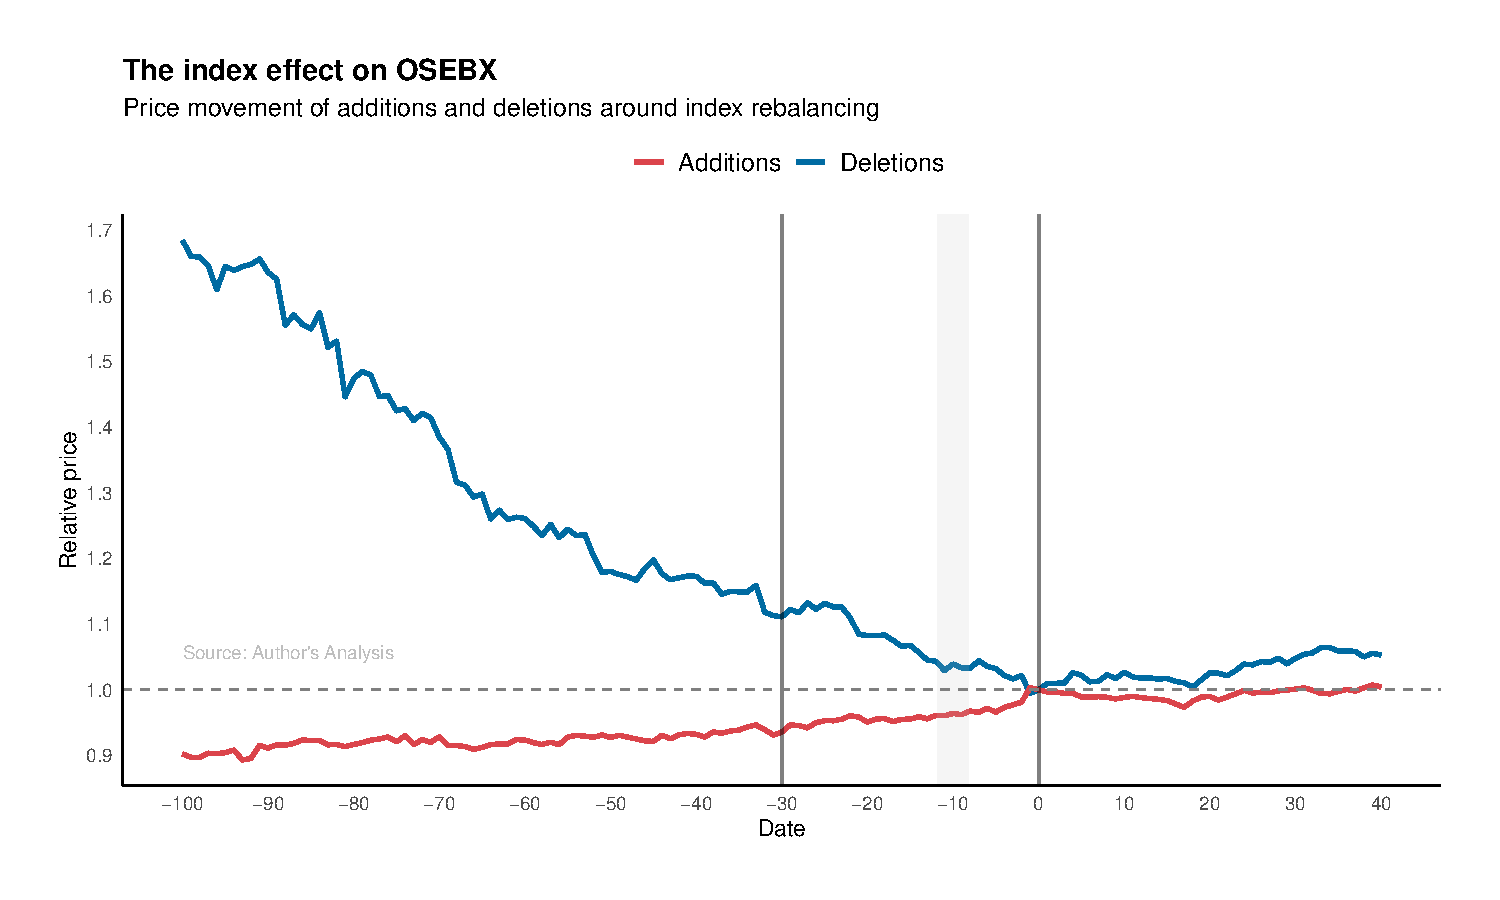
\includegraphics[width=0.8\linewidth]{images/index_plot_updated.pdf}
\caption{\textbf{OSEBX index effect, 2002--2023.} Average relative price paths for future additions and deletions around the effective date (day 0). Prices are Bloomberg VWAP series aggregated across historical rebalancing events.}
\label{fig:idxeff}
\end{figure}

The paper contributes a compact, implementable answer to three questions. First, can upcoming OSEBX membership be predicted out of sample using only rule-book information? Second, do the predictions survive transaction costs, short-borrow charges and monthly risk adjustment? Third, can the signal still matter inside the tighter constraints of an enhanced-index mandate, where active risk is capped by tracking error?

The answer is yes, with an important qualification. Machine learning can forecast OSEBX membership with very high headline accuracy, but the highest-accuracy model is also the least useful one: it simply predicts no change. I therefore treat the task as a portfolio-design problem rather than a pure classification problem. The proposed conditional threshold increases the density of addition and deletion signals, and the resulting XGBoost strategy is the only specification that remains economically meaningful after scaling into a 2\% annual tracking-error enhanced-index portfolio.

The contribution sits at the intersection of three literatures. First, the index-effect literature documents reliable price pressure around scheduled rebalances and motivates the trade idea. Second, an emerging strand of work applies machine learning to portfolio construction, showing that tree-based models can outperform linear baselines once features carry mild non-linearities or interactions \parencite{rouf-stock-market-prediction-using-machine-learning,goodell-artificial-intelligence-and-machine-learning-in-finance}. Third, the enhanced-indexing literature constrains active risk by tracking error and so penalises high-volatility overlays \parencite{ahmed-performance-of-enhanced-index-and-quantitative-equity-funds,nbim-from-passive-to-enhanced}. The novelty here is to fuse the three: a rule-book classifier whose loss function is reshaped to optimise a tracking-error-bounded portfolio rather than headline accuracy.

% --------------------- DATA & METHODOLOGY ----------------------------
\section{Data and Methodology}
\label{sec:data}

\subsection{Data and forecasting design}

The investable universe is OSEAX. For each firm and each semi-annual rebalancing event from January 2006 to March 2023, I construct snapshots 30, 60 and 100 trading days before the effective date. The predictors are intentionally restricted to variables that an external investor can observe before the announcement: trading status, 12-month electronic-order-book turnover trimmed for extreme days, free-float-adjusted market capitalisation, ICB super-sector, and four lags of OSEBX membership. This restriction is central to the design. The model is not trying to reverse-engineer hidden discretionary decisions; it is trying to process the same public rule-book inputs faster and more consistently than a manual screen.

Price returns use VWAP series from Bloomberg and Refinitiv DataStream, which better approximate institutional execution than closing prices \parencite{madhavan-vwap,bloomberg-terminal,lseg-refinitiv}. Norwegian Fama--French factors and the risk-free rate are from \textcite{bernt-fama-french} and \textcite{bernt-risk-free}. After cleaning, the three horizon panels contain 5{,}983, 5{,}924 and 5{,}891 firm-event observations. All reported performance is out of sample: for each test rebalancing, the training set contains only events whose cut-off dates are strictly earlier.

\subsection{Models and conditional threshold}

The first classifier is a binomial logistic GLM,
\begin{equation}
\Pr(Y_{i,t}=1 \mid X_{i,t}) = \frac{\exp(\beta^\top X_{i,t})}{1+\exp(\beta^\top X_{i,t})},
\label{eq:glm}
\end{equation}
where $Y_{i,t}=1$ means that firm $i$ is in OSEBX after rebalancing $t$. The second is XGBoost, a regularised boosted-tree model that can capture non-linear interactions between size, liquidity, sector and past membership \parencite{xgboost-a-scaleable-tree-boosting-system}. Hyperparameters are fixed across folds to avoid turning the backtest into a tuning exercise.

The main methodological issue is class persistence. Most current constituents remain in the index and most non-constituents remain out, so ordinary 0--1 loss rewards a model that predicts no additions or deletions. I therefore replace the standard threshold $\theta$ with a threshold conditioned on prior membership:
\begin{equation}
\theta^{\star}_{i,t} =
\begin{cases}
\theta + \varepsilon, & Y_{i,t-1}=1,\\
\theta - \varepsilon, & Y_{i,t-1}=0,
\end{cases}
\qquad
\hat{Y}_{i,t}=\mathbf{1}\{\hat{p}_{i,t}>\theta^{\star}_{i,t}\}.
\label{eq:cppt}
\end{equation}
With $\varepsilon>0$, a current constituent needs stronger evidence to be classified as staying, while a current non-constituent needs less evidence to be classified as entering. The mechanism is deliberately simple: it trades a small amount of calibration accuracy for more addition and deletion signals. I set $\theta=0.6$ and $\varepsilon=0.2$ on the training data. In the results, XGBB denotes standard XGBoost and XGBC denotes XGBoost with this conditional threshold.

\subsection{Portfolio tests}

For each rebalancing event, predicted additions $\mathcal{A}_t$ are bought and predicted deletions $\mathcal{D}_t$ are shorted at the forecast date, then closed at the effective date. Trade returns are equally weighted:
\begin{equation}
r_t^A =
\frac{1}{|\mathcal{A}_t \cup \mathcal{D}_t|}
\sum_{i \in \mathcal{A}_t \cup \mathcal{D}_t} r_i,
\qquad
r_i^{long}=\frac{p_1-p_0}{p_0},\quad
r_i^{short}=\frac{p_0-p_1}{p_0}.
\label{eq:retdef}
\end{equation}
The active simulation applies 4 bps per leg in transaction costs \parencite{dnb-transaction-costs}, a 4\% annual short-borrow charge \parencite{nordnet-short-interest-rate}, and a forced buy-back cap at a 100\% short loss. Outside active event windows the capital is invested in OSEBX.

The enhanced-index version combines OSEBX with the active sleeve:
\begin{equation}
r_t^E=s r_t^A+(1-s)r_t^{OSEBX},
\label{eq:enhanced}
\end{equation}
where $s$ is the largest realised weight that keeps annual tracking error below 2\%, a common enhanced-index risk budget \parencite{ssg-tracking-error-enhanced}. In this version, shorted deletion names are treated as sales from the passive inventory, so the short-borrow charge is removed. Risk-adjusted performance is measured with CAPM and Norwegian Fama--French three-factor regressions over January 2010 to May 2022, the longest period with factor data.

% --------------------- EMPIRICAL RESULTS -----------------------------
\section{Empirical Results}
\label{sec:results}

\subsection{Prediction: accuracy is not enough}

Table~\ref{tab:acc} reports out-of-sample classification performance over 26 rebalancing events. The rule-book variables contain strong signal: every learned model has AUROC above 0.97, even 100 trading days before the effective date. However, accuracy alone gives the wrong investment ranking. The naive model that simply repeats last period's membership has the highest accuracy, 95.07\%, but predicts no changes and therefore cannot be traded.

\begin{table}[H]
\centering
\footnotesize
\begin{tabular}{lccccccc}
\toprule
Model & Acc. & Prec. & Sens. & Spec. & F & AUROC & Pred.\ changes \\
\midrule
\texttt{index\_lag1} & 0.9507 & 0.9208 & 0.9399 & 0.9565 & 0.9303 & 0.9446 & 0 \\
\midrule
GLM-100  & 0.9506 & 0.9292 & 0.9328 & 0.9605 & 0.9310 & 0.9789 & 63  \\
GLM-60   & 0.9497 & 0.9293 & 0.9298 & 0.9607 & 0.9296 & 0.9808 & 76  \\
GLM-30   & 0.9482 & 0.9259 & 0.9288 & 0.9589 & 0.9274 & 0.9797 & 93  \\
XGBB-30  & 0.9398 & 0.9316 & 0.9030 & 0.9613 & 0.9171 & 0.9812 & 174 \\
XGBB-60  & 0.9408 & 0.9331 & 0.9043 & 0.9621 & 0.9184 & 0.9817 & 165 \\
XGBC-30  & 0.9260 & 0.9208 & 0.8780 & 0.9548 & 0.8989 & 0.9812 & 271 \\
XGBC-60  & 0.9317 & 0.9318 & 0.8834 & 0.9609 & 0.9069 & 0.9817 & 247 \\
\bottomrule
\end{tabular}
\caption{\textbf{Out-of-sample prediction performance, 2010--2023.} Representative model-horizon combinations. ``Pred.\ changes'' is the total number of predicted additions plus deletions. XGBB is standard XGBoost; XGBC applies the conditional threshold in equation~(\ref{eq:cppt}).}
\label{tab:acc}
\end{table}

The conditional threshold does what it is designed to do. XGBC-30 reduces accuracy by 1.4 percentage points relative to XGBB-30, but increases predicted changes from 174 to 271. This is not a cosmetic difference: an index-event strategy earns nothing from correctly predicting that Equinor remains in the benchmark. It earns from the small set of names whose membership changes, and the model must create enough of those signals to diversify event risk.

\subsection{Active long--short overlays}

The active strategy confirms that prediction quality translates into investable return, but through two different channels. Table~\ref{tab:ff3} summarises monthly performance over the factor-test window. OSEBX earned 0.95\% per month with 4.23\% volatility. GLM-60 and GLM-100 produce the highest excess returns, but they do so with concentrated books and high volatility. XGBC-30 produces lower raw excess return, but is closer to the benchmark in beta and tracking error.

\begin{table}[H]
\centering
\footnotesize
\setlength{\tabcolsep}{3.5pt}
\begin{tabular}{lcccccccc}
\toprule
Portfolio & $R_p-R_b$ & $R_p$ & $\sigma_p$ & SR & $\alpha_{CAPM}$ & $\beta$ & TE$_{ann}$ & $\alpha_{FF3}$ \\
\midrule
OSEBX   & 0.0000 & 0.0095 & 0.0423 & 0.198 & 0.0002 & 1.015 & 0.000 & 0.001 \\
\midrule
GLM-60  & \textbf{0.0095} & 0.0190 & 0.0756 & 0.237 & 0.0139 & 0.497 & 0.260 & \textbf{0.013$^{**}$} \\
GLM-30  & 0.0034 & 0.0129 & 0.0511 & 0.231 & 0.0048 & 0.863 & 0.126 & \textbf{0.006$^{**}$} \\
XGBC-30 & 0.0017 & 0.0112 & 0.0441 & 0.229 & 0.0026 & 0.925 & 0.079 & \textbf{0.004$^{**}$} \\
GLM-100 & 0.0087 & 0.0182 & 0.0757 & 0.226 & 0.0133 & 0.468 & 0.267 & \textbf{0.013$^{**}$} \\
XGBB-30 & 0.0010 & 0.0105 & 0.0488 & 0.192 & 0.0016 & 0.954 & 0.106 & 0.003 \\
XGBC-60 & $-$0.0029 & 0.0066 & 0.0480 & 0.114 & $-$0.0004 & 0.729 & 0.138 & 0.001 \\
\bottomrule
\end{tabular}
\caption{\textbf{Active long--short overlays, monthly returns, January 2010--May 2022.} Alphas use OSEAX as the market proxy and Norwegian Fama--French factors. $^{**}$ denotes $p<0.05$.}
\label{tab:ff3}
\end{table}

\begin{figure}[H]
\centering
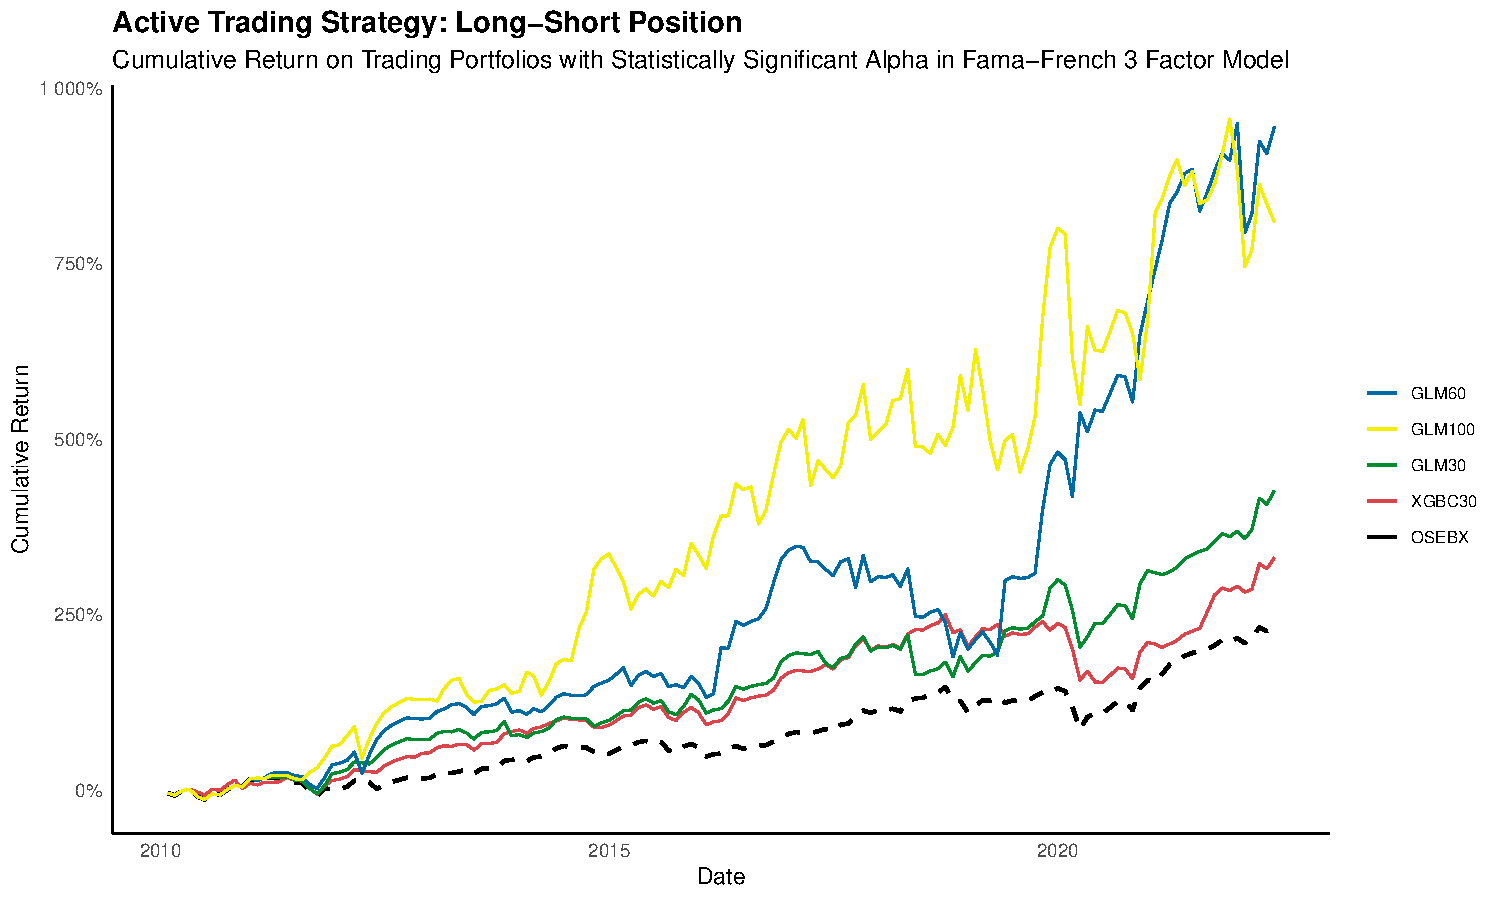
\includegraphics[width=0.78\linewidth]{images/trading_long_short.pdf}
\caption{\textbf{Cumulative active strategy returns.} Four active overlays with significant FF3 alpha compared with OSEBX. Initial capital is 1 NOK; transaction costs and short-borrow assumptions are included.}
\label{fig:cumret_active}
\end{figure}

For a discretionary active mandate, the GLM portfolios are attractive because they extract more return from fewer, cleaner signals. For a benchmarked mandate, the more important result is XGBC-30: it earns significant alpha while keeping annual tracking error below 8\% before any enhanced-index scaling. That lower active risk is what gives the signal capacity in the next test.

\subsection{Enhanced-index implementation}

The enhanced-index test is the stricter and more commercially relevant version. Each active overlay is scaled to the largest weight consistent with 2\% annual tracking error against OSEBX. This constraint sharply penalises concentrated portfolios: GLM-60 can only receive a 4.1\% active weight, while XGBC-30 can receive 22.1\%. After scaling, the ranking reverses. GLM still adds some raw return, but only XGBC-30 produces a positive FF3 alpha that is statistically distinguishable from zero at the 10\% level.

\begin{figure}[H]
\centering
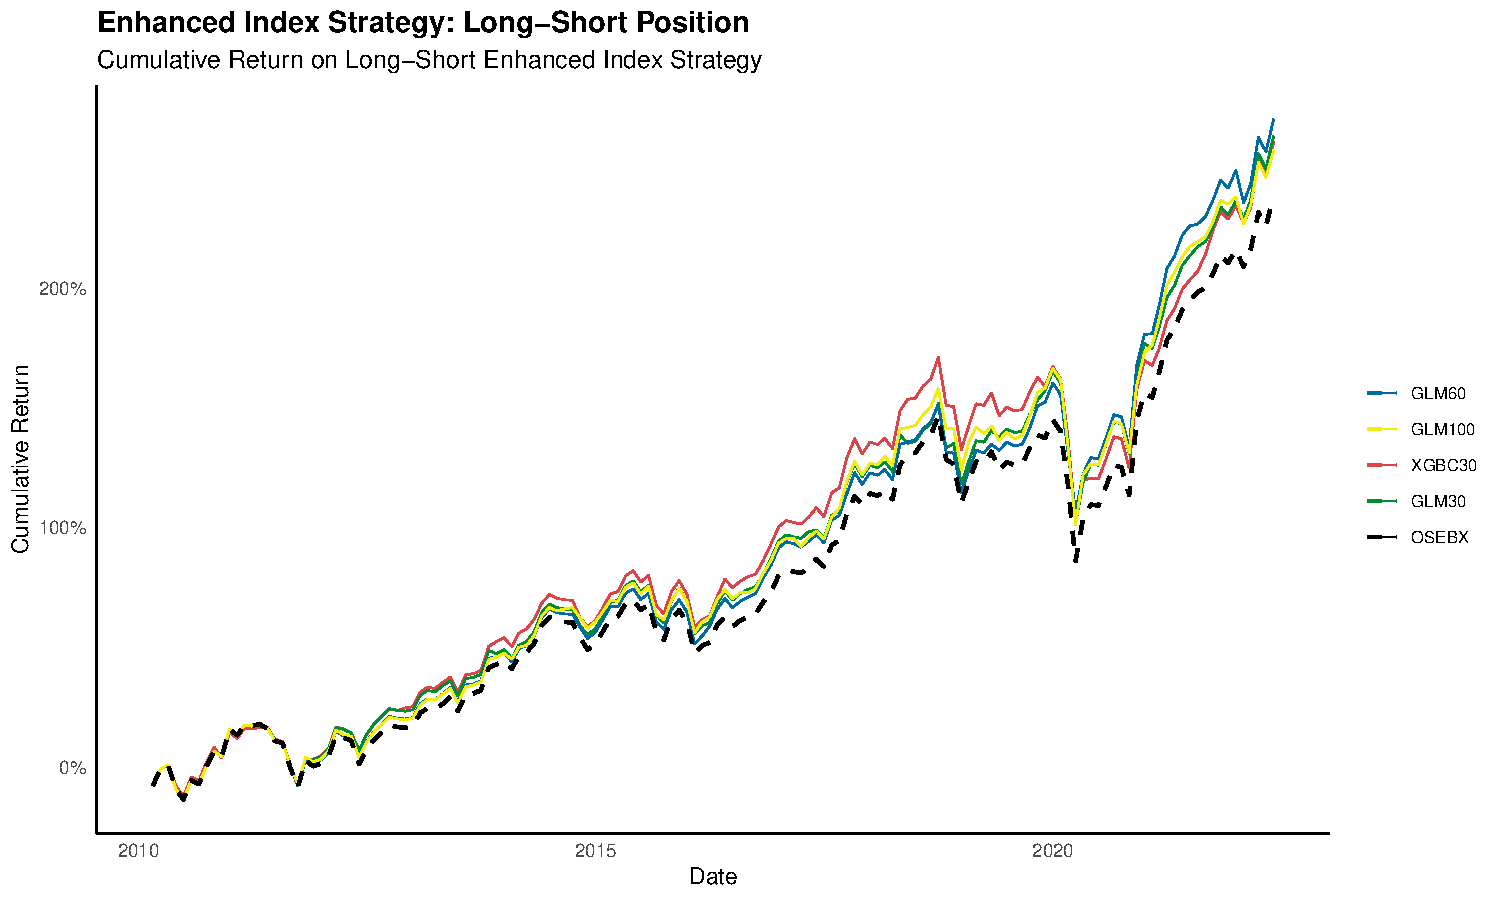
\includegraphics[width=0.78\linewidth]{images/enhanced_long_short.pdf}
\caption{\textbf{Enhanced-index portfolios.} Active overlays are combined with OSEBX and scaled to 2\% annual tracking error. XGBC-30 is the only long--short enhanced variant with significant FF3 alpha.}
\label{fig:cumret_enh}
\end{figure}

This is the practical finding. The same forecast that looks slightly worse in a classification table becomes the better product candidate once the portfolio is constrained like an enhanced-index fund. The threshold in equation~(\ref{eq:cppt}) is therefore not just a statistical tweak; it is a way to align the classifier with the economic objective.

% ------------------------ CONCLUSION ---------------------------------
\section{Conclusion}
\label{sec:conc}

OSEBX rebalancing is predictable and partly tradable before the official announcement date. Using only public Euronext rule-book variables, GLM and XGBoost models achieve AUROC above 0.97 across the 2010--2023 out-of-sample window. More importantly, portfolios formed from predicted additions and deletions generate economically meaningful alpha after transaction costs, short-borrow costs and factor adjustment.

The strongest lesson is that model selection must follow the investment objective. The naive persistence model is the most accurate classifier but creates no portfolio. The conditional-threshold XGBoost model is less accurate, yet produces more diversified event exposure and is the only specification that remains significant inside a realistic 2\% tracking-error enhanced-index sleeve. For a portfolio manager, that is the relevant victory: a repeatable signal that can be scaled inside a benchmarked risk budget.

The result is bounded by three caveats. First, the Norwegian factor data end in May 2022, so the latest rebalancing events are included in classification and portfolio plots but not in the FF3 regressions. Second, the cost assumptions are institutional; retail implementation would face wider spreads, higher commissions and less reliable short access. Third, the index effect can decay as arbitrage capital learns the rule. The natural extension is therefore a live paper-trading implementation over the next five OSEBX rebalances, with pre-registered thresholds and execution rules. Subject to those caveats, the strategy is implementable today with public index methodology, standard market data and an open-source machine-learning workflow.

\newpage
\printbibliography[heading=bibintoc,title={References}]
\newpage
\appendix
% ----------------------------- APPENDIX ------------------------------
\section{Appendix}
\label{app:diagnostics}

% Optional: slightly tighter appendix figure captions
\captionsetup[figure]{font=footnotesize,labelfont=bf,skip=4pt}

% Optional: common appendix figure width
\newcommand{\appfigwidth}{0.7\linewidth}

\begin{figure}[H]
    \centering
    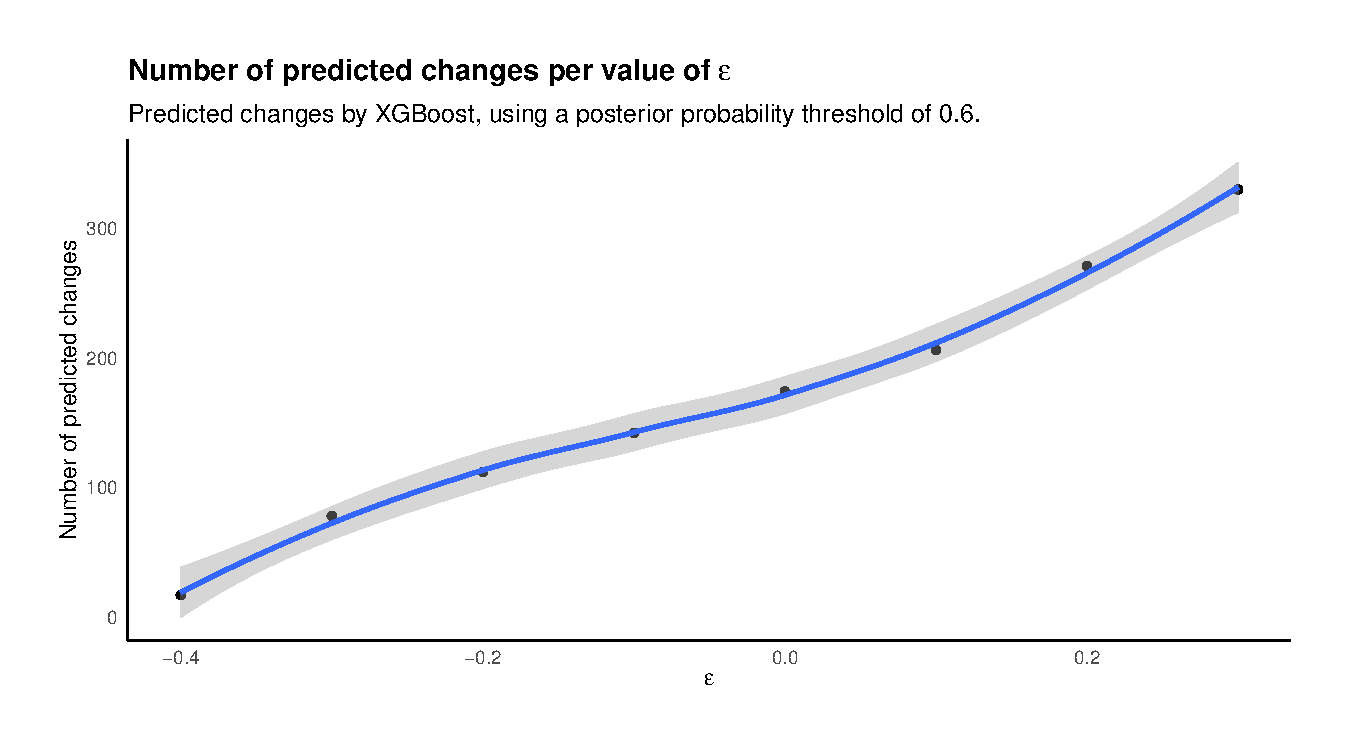
\includegraphics[width=\appfigwidth]{images/beta_plot.pdf}
    \caption{\textbf{Conditional-threshold calibration.}
    Predicted index changes as the conditional-threshold parameter $\varepsilon$ varies.
    The diagnostic shows why $\varepsilon=0.2$ is a pragmatic compromise: it materially increases signal count without pushing the strategy toward indiscriminate turnover.}
    \label{fig:app_beta}
\end{figure}

\begin{figure}[H]
    \centering
    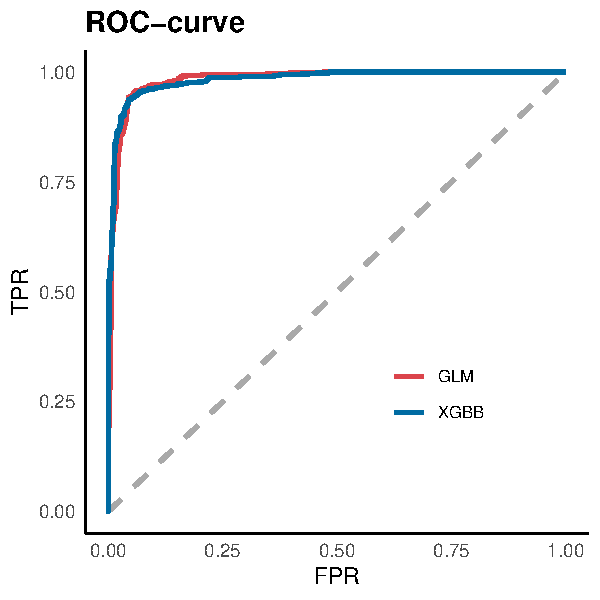
\includegraphics[width=0.5\textwidth]{images/roc_curve.pdf}
    \caption{\textbf{ROC curves for benchmark forecasts.}
    ROC curves for the 30-day GLM and XGBoost forecasts.
    The curve confirms that the underlying probability rankings remain informative before the announcement date, even when the final trading rule must still handle class imbalance and signal scarcity.}
    \label{fig:app_roc}
\end{figure}

\begin{figure}[H]
    \centering
    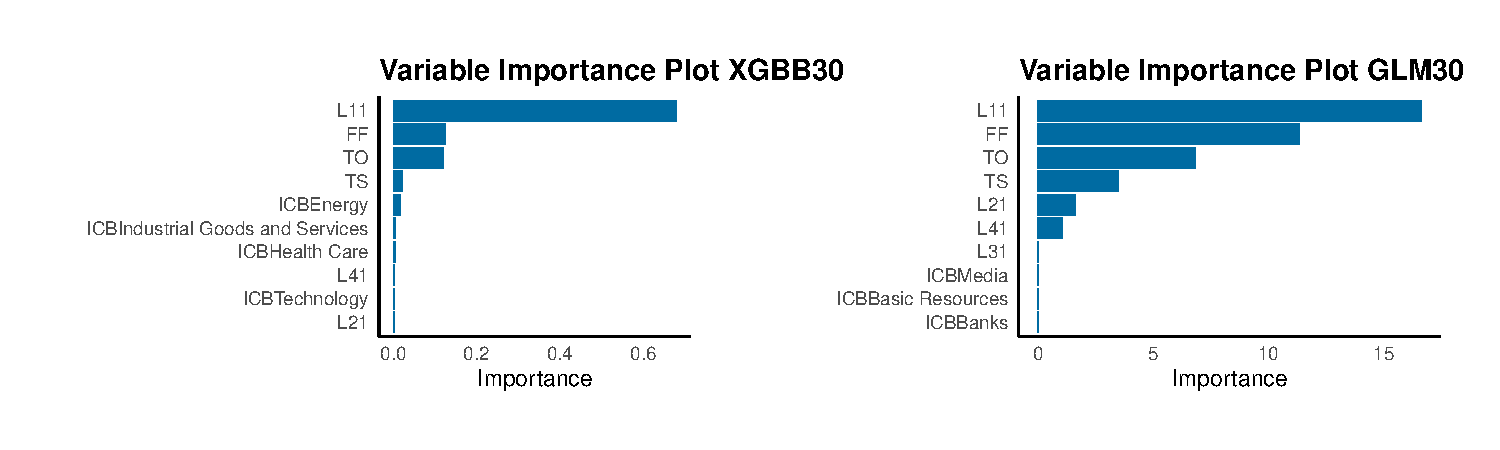
\includegraphics[width=\textwidth]{images/vip.pdf}
    \caption{\textbf{Variable importance for 30-day forecasts.}
    Lagged index membership dominates both models, while free float, turnover, trading status, and sector classification supply the marginal information needed to identify additions and deletions.}
    \label{fig:app_vip}
\end{figure}

\begin{figure}[H]
    \centering
    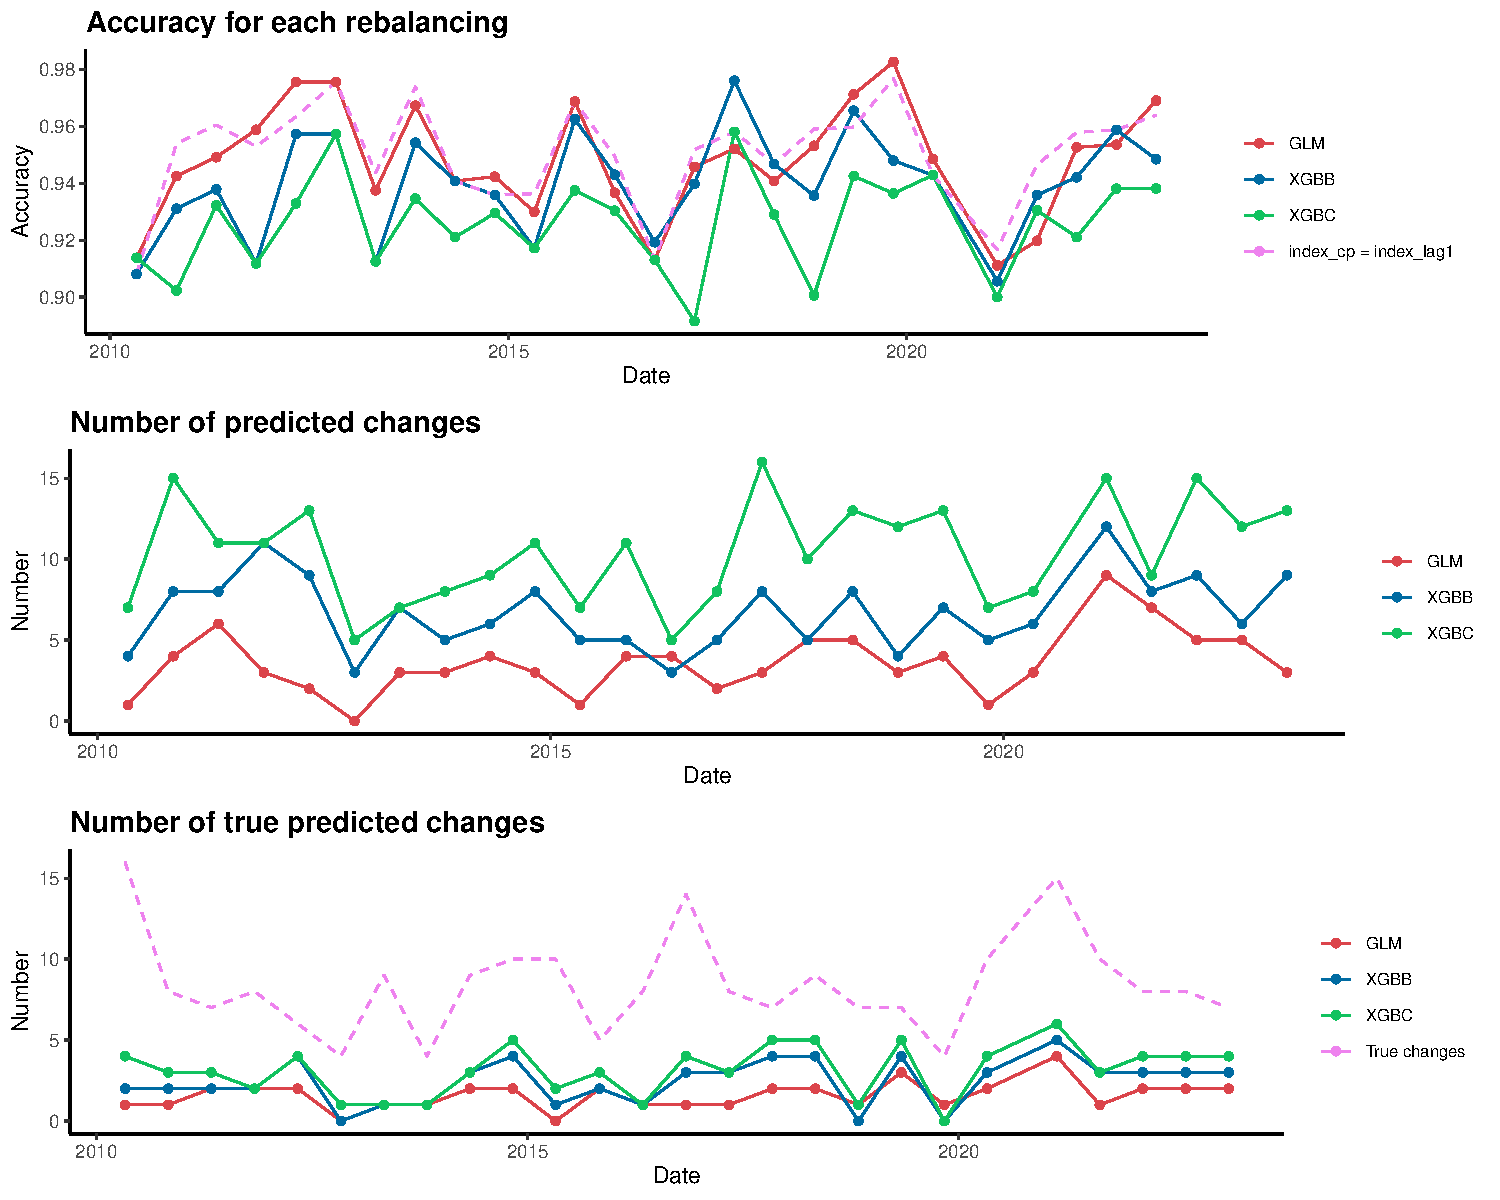
\includegraphics[width=\appfigwidth]{images/machinelearning_res.pdf}
    \caption{\textbf{Prediction performance through time.}
    Period-by-period accuracy, predicted changes, and captured changes for the 30-day GLM, XGBB, and XGBC specifications.
    The figure highlights the recurring trade-off between maximum classification accuracy and economically useful signal density.}
    \label{fig:app_ml_time}
\end{figure}

\begin{figure}[H]
    \centering
    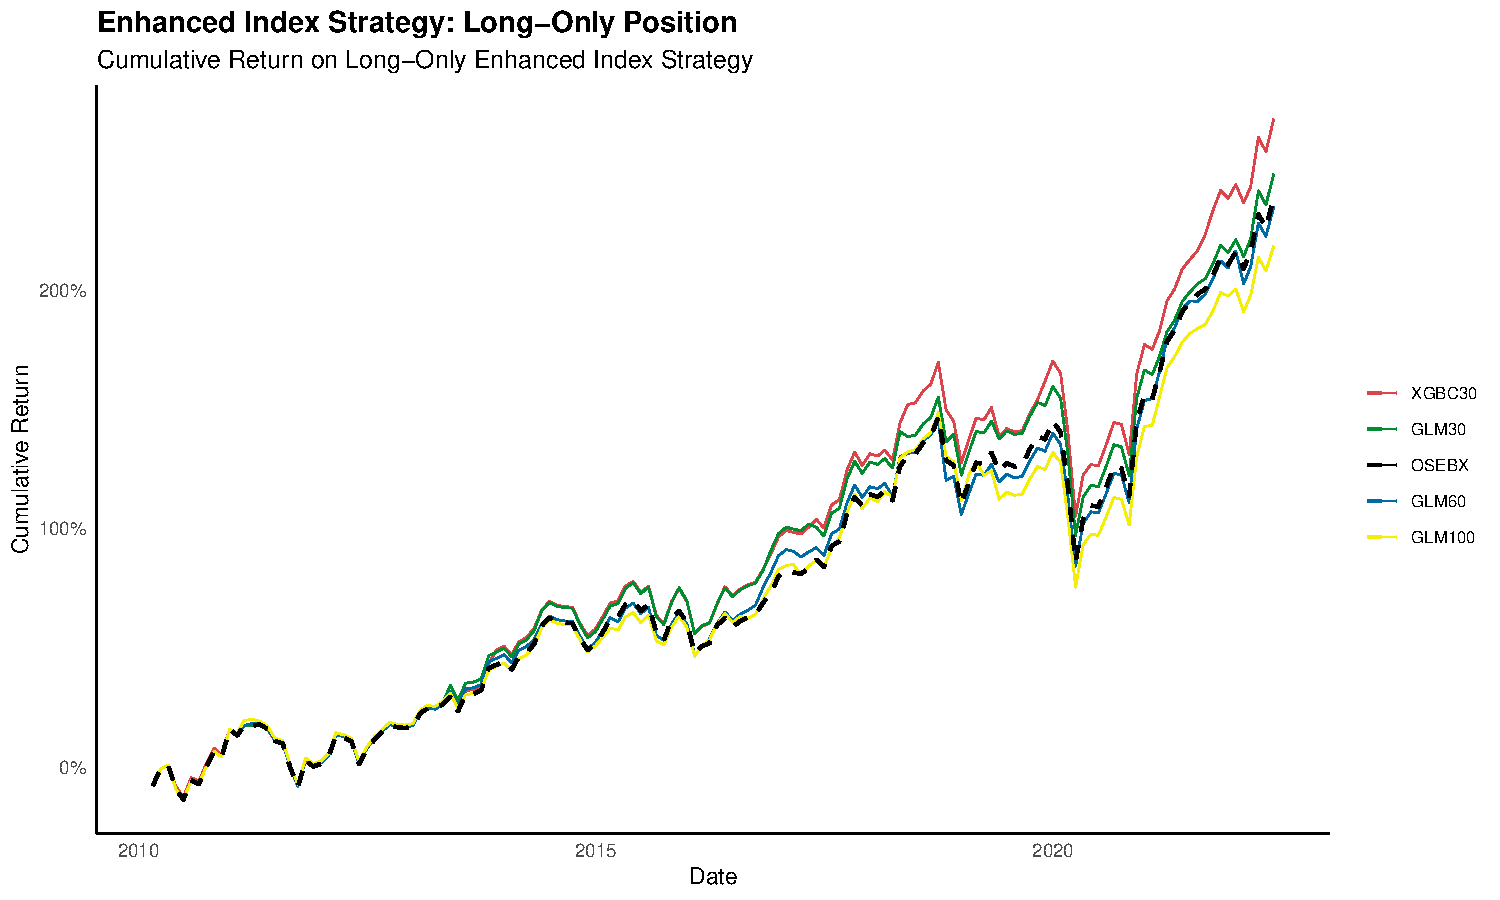
\includegraphics[width=\appfigwidth]{images/enhanced_long_only.pdf}
    \caption{\textbf{Long-only enhanced-index robustness check.}
    Long-only overlays also track OSEBX closely after scaling to the 2\% tracking-error budget, but none generates significant FF3 alpha in the thesis backtest.
    This supports the paper's focus on the long--short XGBC-30 variant.}
    \label{fig:app_enhanced_long_only}
\end{figure}

\end{document}
